%5_1.tex

実装した命令が正しく出力されるか,図\ref{fig:add_array_c}
に示した配列加算のプログラムを入力としてアセンブリコードの出力を行う.図\ref{fig:add_array_c}は配列要素数999の配列aおよび配列bの各要素の加算結果を配列cに格納する配列加算プログラムである.
生成はまずコマンド\textit{clang -O3 add\_array.c -emit-llvm -S -mllvm -force-vector-width=4}を用いてLLVMのC ,C++向けフロントエンドClangによるベクトル化LLVM IRの生成を行う.オプション\textit{-O3}は最適化レベルの設定であり,自動ベクトル化を行うために設定する.\textit{-emit-llvm} ,\textit{-S}を設定することでLLVM IRで出力が行われる.\textit{-mllvm} ,\textit{-force-vector-width=4}は自動ベクトル化を行う際のベクトル命令で演算を行う配列要素数の設定を行い,その数を4に設定している.
アセンブリコードの生成はLLVM IRからアセンブリコードへのコンパイラであるllcを用いて行う.コマンドは\textit{llc add\_array.ll -mattr=experimental-v -riscv-v-vector-bits-min=128}を実行した.オプション\textit{-mattr=experimental-v}はベクトル化LLVM IRからベクトル化アセンブリコードを生成する機能の有効かを行っており,\textit{-risc-v-vector-bits-min=128}はベクトルレジスタの幅の最小値の指定を行っており,ベクトル拡張付きRISC-Vのベクトルレジスタの最小値である128ビットを設定している.

\begin{figure}[tb]
    \centering
    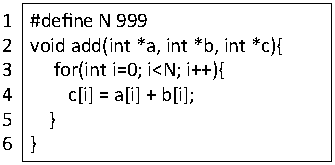
\includegraphics[scale=1.2]{image/add_array_c.pdf}
    \caption{配列加算プログラム}
    \label{fig:add_array_c}
\end{figure}

図\ref{fig:rv_vectorized_assembly}は配列a,bの各要素の加算した結果を配列cに格納する関数addのアセンブリコードである.
25行目にあるベクトル加算命令\textit{vadd.w}が実装の対象となる命令である.21行目から31行目にてベクトル演算を行っている.23 ,34行目にてベクトル加算を行うデータのロードを行っており,25行目にてロードしたデータの加算を行い,26行目にて加算結果のストアを行っている.27行目では20行目で設定したループカウンタを演算を行った配列要素数分デクリメントをしている.
32行目から37行目では余りの要素の逐次処理を行っている.33行目で演算対象配列の全要素数からベクトル処理対象の配列要素数を減算することで余りの要素数を計算し,余りの要素数分配列要素の加算を行う.

\begin{figure}
    \centering
    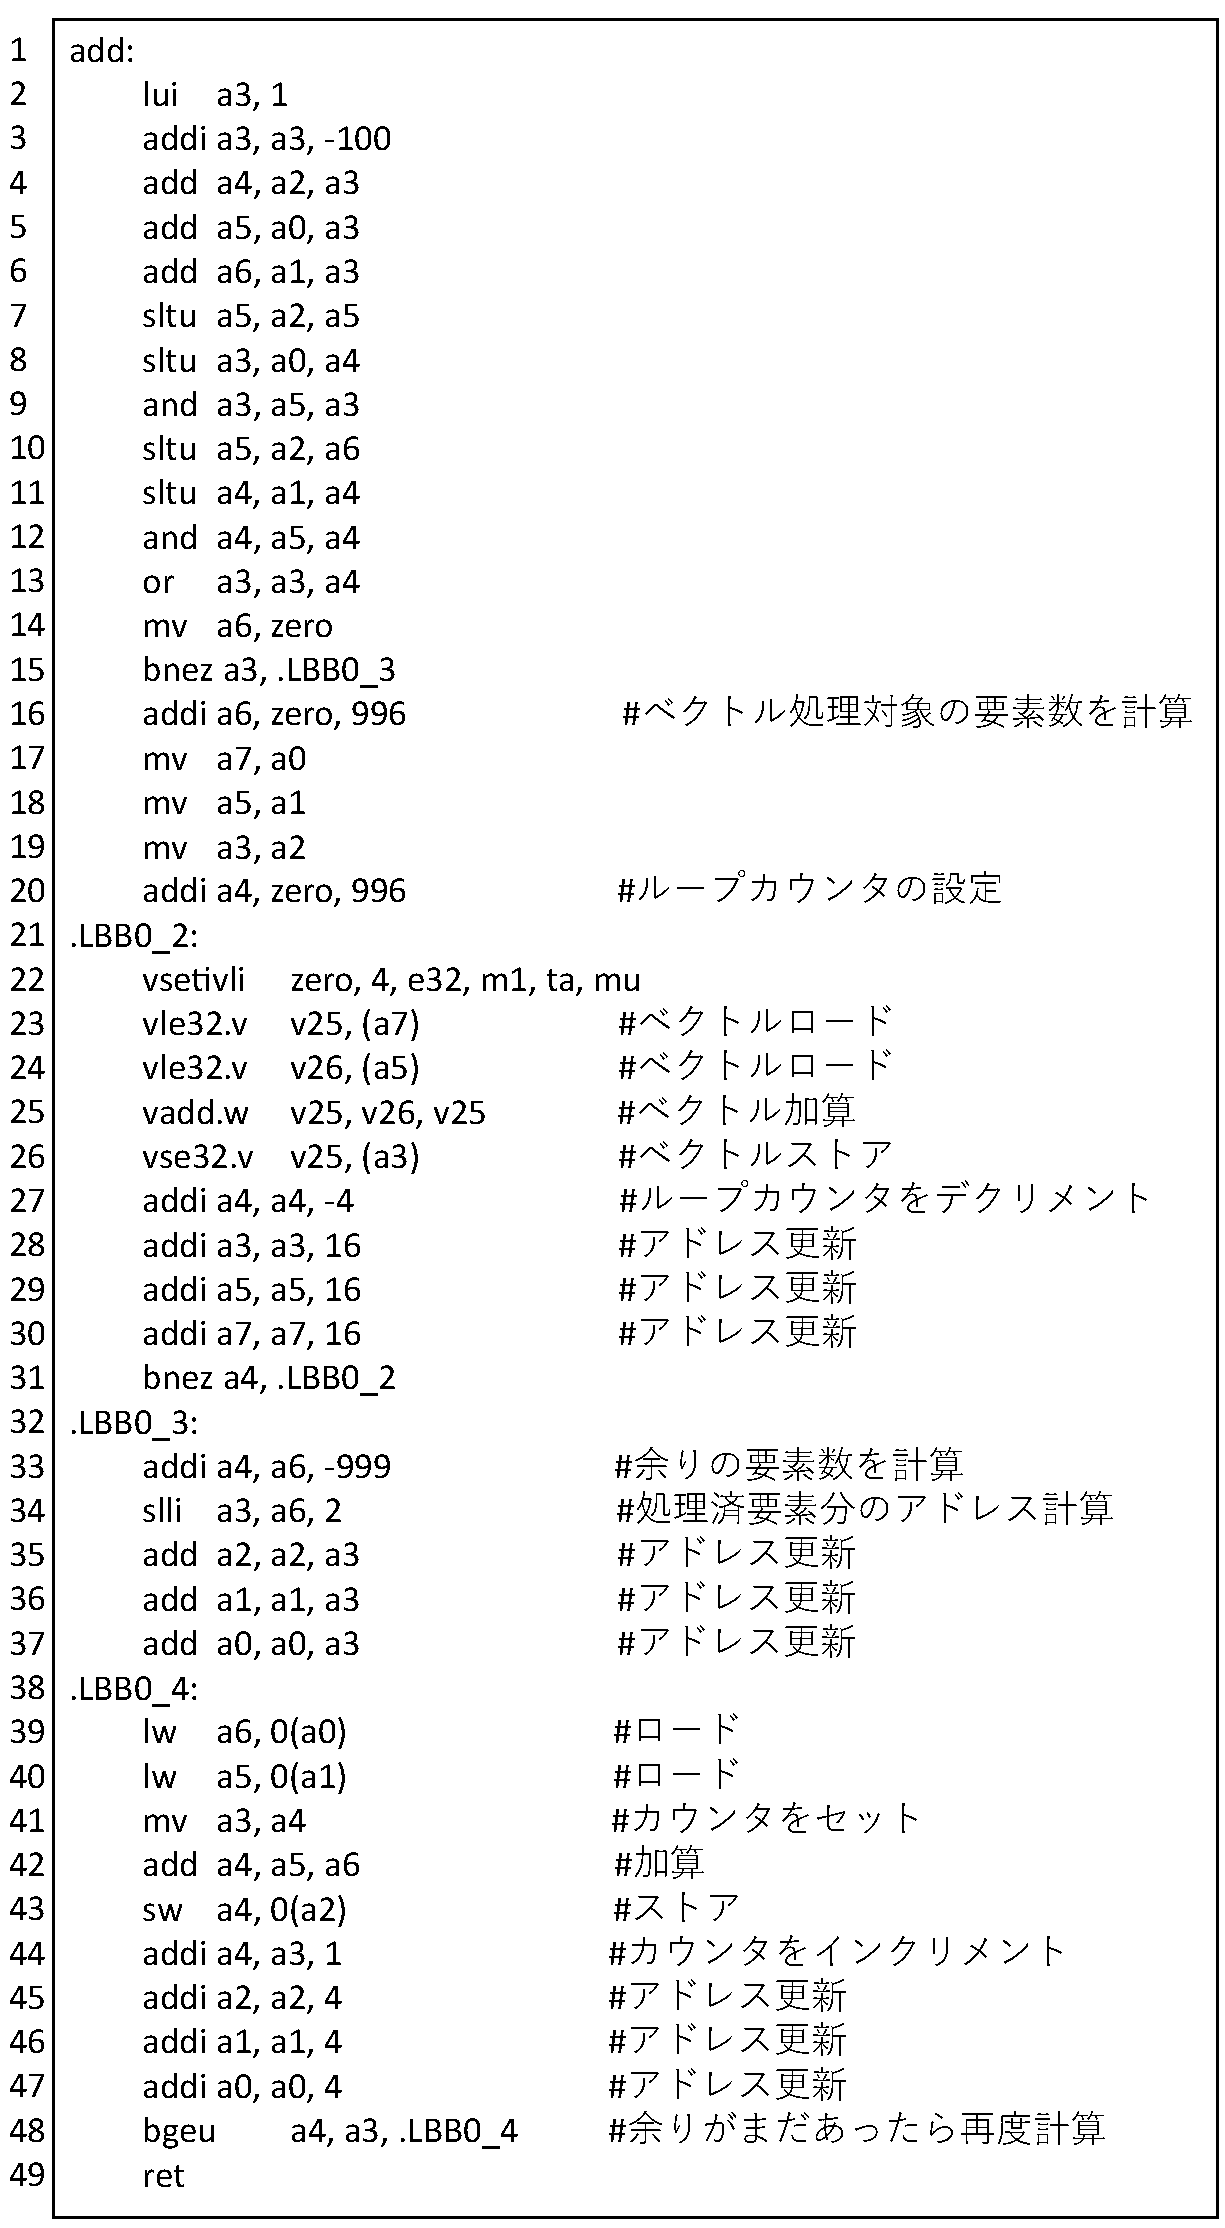
\includegraphics[scale=0.55]{image/rv_vectorized_assembly.pdf}
    \caption{生成されたアセンブリコード}
    \label{fig:rv_vectorized_assembly}
\end{figure}

図\ref{fig:add_array_c}の配列要素加算部分を変更し,他の定義した命令の生成を検証する.

ベクトル減算命令であるvsubの生成を図\ref{fig:vsub}
に,
ベクトル論理積,ベクトル論理和,ベクトル排他的論理和命令であるvand ,vor ,vxorの生成を図\ref{fig:vand},図\ref{fig:vor},図\ref{fig:vxor}に示す.図\ref{fig:vsub},\ref{fig:vand},図\ref{fig:vor},図\ref{fig:vxor}では実装対象の命令の生成確認のためにC言語で記述されるプログラム内の配列要素の演算箇所の演算子を変更している.

また,即値を用いたベクトル演算命令の生成も検証した.
即値によるベクトル加算・減算命令の生成を図に示す.定数を指定して配列要素への加算を行うプログラムを入力することで即値による加算命令となる.

同様に即値を用いる論理演算命令についてもvandiを図\ref{fig:vandi}
にvoriを図\ref{fig:vori}
にvxoriを図\ref{fig:vxori}
に示す.

即値によるベクトルシフト演算命令について,ベクトル論理左シフト命令であるvsllを図\ref{fig:vsll}
に示す.ベクトル算術右シフト命令であるvsraを図\ref{fig:vsra}
に示す.ベクトル論理右シフト命令であるvsrlを図\ref{fig:vsrl}
し示す.ベクトル論理右シフト命令を出力するためにC言語で記述したプログラムないの演算対象の配列の型宣言をint型から符号なし整数型であるunsigned intに変更している.論理シフト演算は符号ビットが考慮されないシフト演算命令出るため,符号付き整数型であるint型から符号なし整数型であるunsigned intに変更することによって論理シフト命令の生成を可能にしている.

\begin{figure}
    \centering
    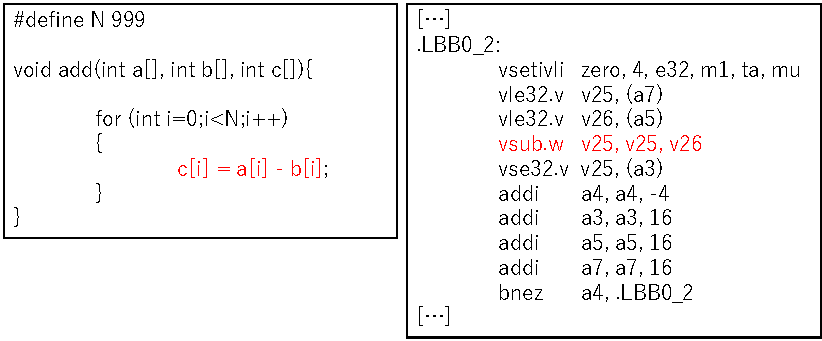
\includegraphics[scale=0.8]{image/vsub.pdf}
    \caption{vsub命令の生成}
    \label{fig:vsub}
\end{figure}

\begin{figure}
    \centering
    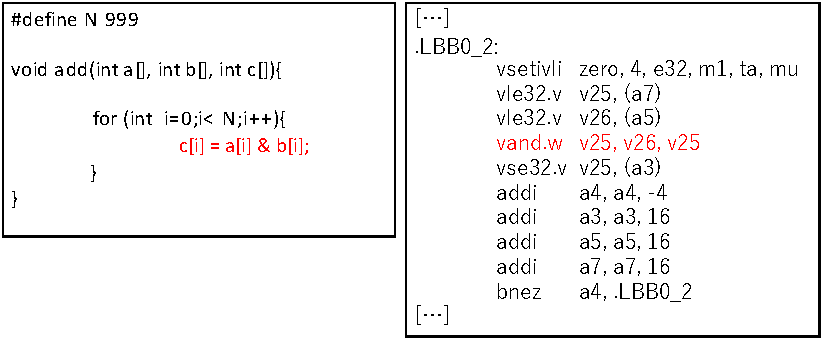
\includegraphics[scale=0.8]{image/vand.pdf}
    \caption{vand命令の生成}
    \label{fig:vand}
\end{figure}

\begin{figure}
    \centering
    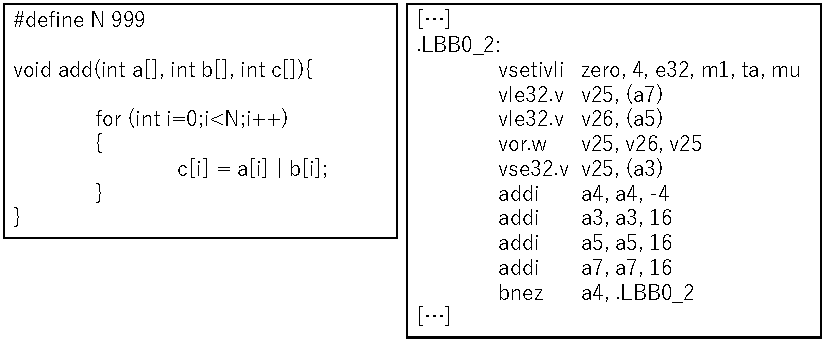
\includegraphics[scale=0.8]{image/vor.pdf}
    \caption{vor命令の生成}
    \label{fig:vor}
\end{figure}

\begin{figure}
    \centering
    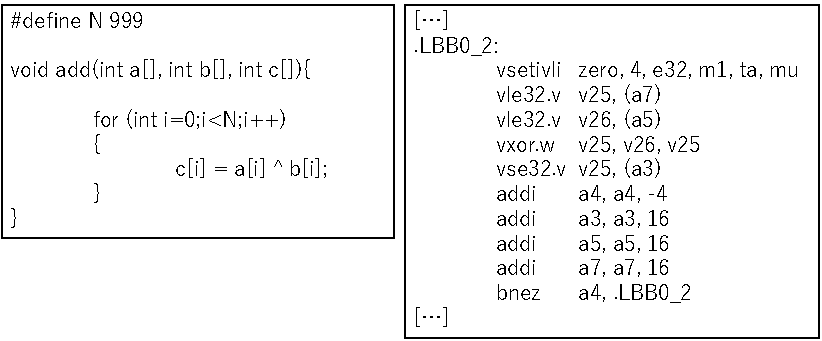
\includegraphics[scale=0.8]{image/vxor.pdf}
    \caption{vxor命令の生成}
    \label{fig:vxor}
\end{figure}

\begin{figure}
    \centering
    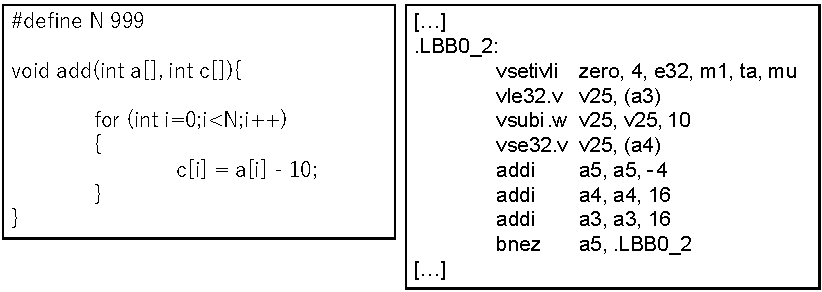
\includegraphics[scale=0.8]{image/vsubi.pdf}
    \caption{vsubi命令の生成}
    \label{fig:vsubi}
\end{figure}

\begin{figure}
    \centering
    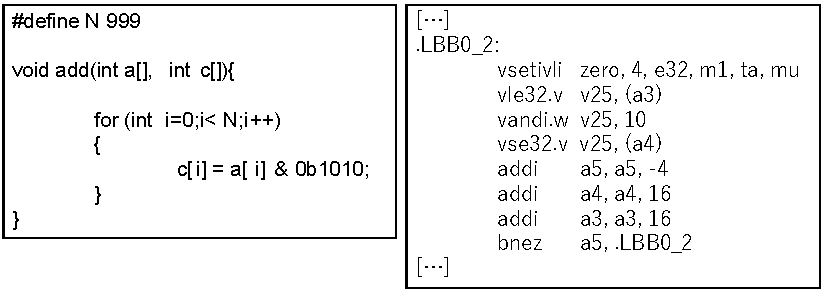
\includegraphics[scale=0.8]{image/vandi.pdf}
    \caption{vandi命令の生成}
    \label{fig:vandi}
\end{figure}

\begin{figure}
    \centering
    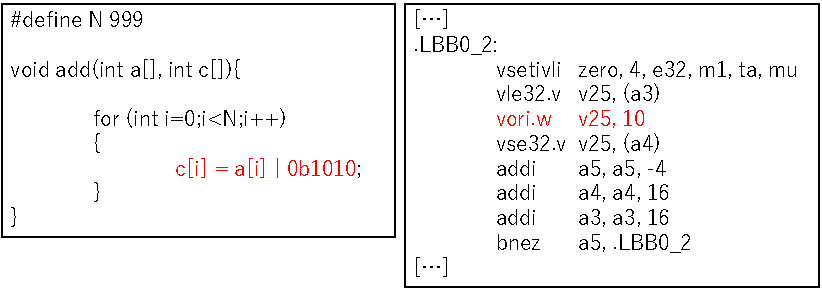
\includegraphics[scale=0.8]{image/vori.pdf}
    \caption{vori命令の生成}
    \label{fig:vori}
\end{figure}

\begin{figure}
    \centering
    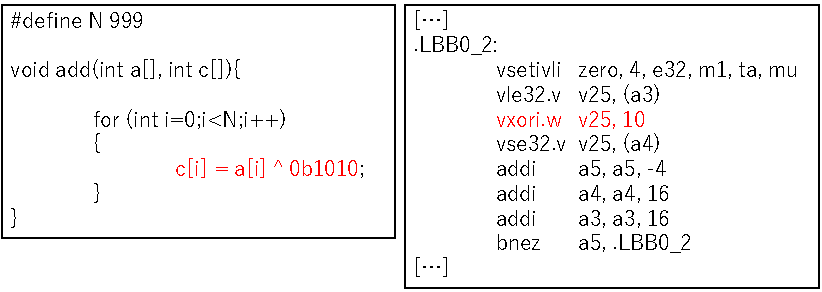
\includegraphics[scale=0.8]{image/vxori.pdf}
    \caption{vxori命令の生成}
    \label{fig:vxori}
\end{figure}

\begin{figure}
    \centering
    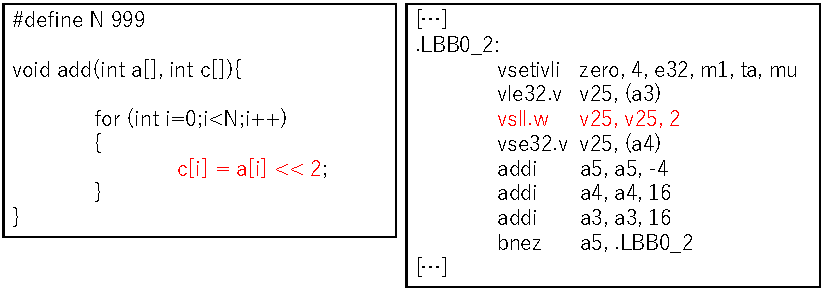
\includegraphics[scale=0.8]{image/vsll.pdf}
    \caption{vsll命令の生成}
    \label{fig:vsll}
\end{figure}

\begin{figure}
    \centering
    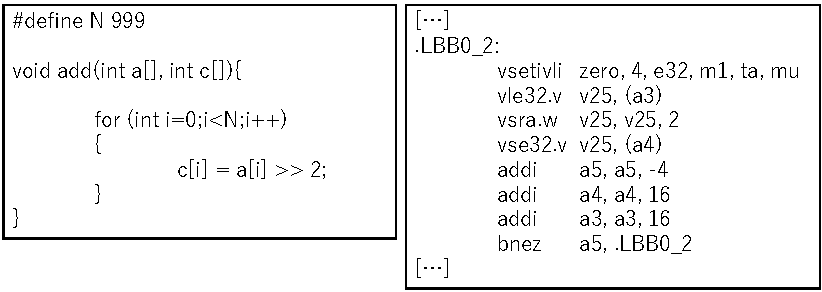
\includegraphics[scale=0.8]{image/vsra.pdf}
    \caption{vsra命令の生成}
    \label{fig:vsra}
\end{figure}

\begin{figure}
    \centering
    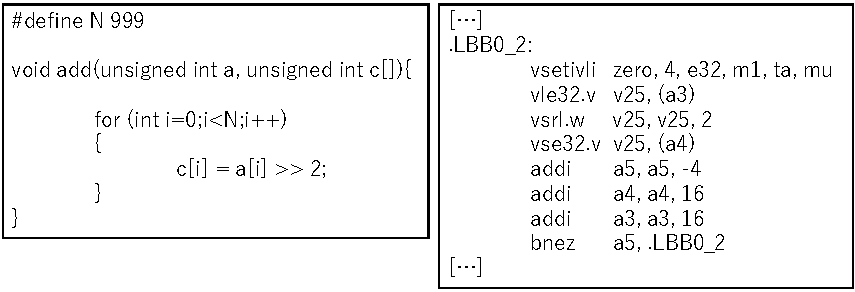
\includegraphics[scale=0.8]{image/vsrl.pdf}
    \caption{vsrl命令の生成}
    \label{fig:vsrl}
\end{figure}